In this section, two new evaluative model architectures are explained. The grasp generator model, given in the previous section, requires very little training data to train. It can generate 1000 candidate grasps, ranked according to their estimated likelihoods, within 20 seconds on a 2x Intel Xeon E5-2650 v2 Eight Core 2.6GHz. The generative model does not estimate a probability of success for the generated grasps. An evaluative model, which is a Deep Neural Network (DNN), is used specifically for this purpose. DNNs have shown good performances in learning to evaluate grasps using grippers \cite{Levine1, Lenz2015} and dexterous hands \cite{Varley2017, lu2017planning}. 

The generative method ignores the global information about the object, such as the overall shape and the object class, to a large extent. It takes the robot hand model and the local object shape features into account. Moreover, it only has access to the partial object shape, due to the noise in the image acquisition process and self-occlusions. The success of an executed grasp, however, depends on other factors such as the full object shape, mass, mass distribution, surface friction and deformability, among others. An evaluative network indirectly learns the effect of these parameters on the grasp outcome. The data provided to the evaluative network is collected from randomly generated scenes, therefore each scene has a different random combination of the parameters. The primary purpose of the network is to learn robust grasps across different conditions, and this is a complex task. The first challenge is that the kinematic model of the hand is unknown to the evaluative network. It only has access to the parameters that \textit{configure} the hand: the wrist and joint positions. Second, the system is weakly supervised with the grasp result (success or failure), and no further labels are provided.

Both proposed evaluative models have similar characteristics. The evaluative DNN based on the VGG-16 network \cite{Simonyan14c}, named Evaluative Model 1 (EM1), is given in Figure \ref{fig:networkArchitecture}. A slightly different version based on the ResNet-50 network, termed Evaluative Model 2 (EM2), is shown in Figure \ref{fig:ResNet}. \footnote{The design of the networks belongs to the author. They were implemented and trained in TensorFlow by Chao Zhao, a MSc student collaborating with Umit Rusen Aktas and Prof. Jeremy L. Wyatt. } Regardless of the type, a grasp evaluation network has the functional form $f(I_t, h_t)$, where $I_t$ is a colourised depth image of the object, and $h_t$ contains a series of wrist poses and joint configurations for the hand, converted to the camera's frame of reference. The network's output layer calculates a probability of success for the image-grasp pair $I_t$, $h_t$. The model initially processes the grasp parameters and visual information in separate channels, and combines them to learn the final output. 

\begin{figure}[h]
  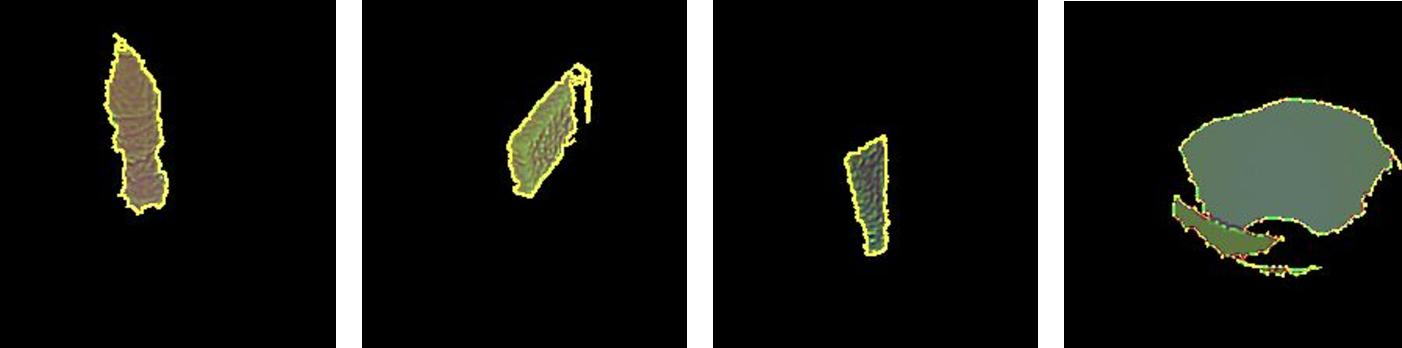
\includegraphics[width=0.9\linewidth]{images/colourDepth.pdf}
  \caption[Colourised depth images.]{Colourised depth images. From left to right, the objects are: coke bottle, chocolate box, hand cream, and bowl.}
\label{fig:colorisedDepth}
\end{figure}

The depth image is colourised before it is passed as input to the evaluative network. The colorisation process converts the single-channel depth data to a 3-channel RGB image. We first crop the middle $460 \times 460$ section of the $640 \times 480$ depth image, and downsample it to $224 \times 224$. Then, two more channels of information are added: mean and Gaussian curvatures, obtained from the object's surfaces in the image. Figure \ref{fig:colorisedDepth} contains four examples of colourised depth images. This procedure both provides a meaningful set of features to the network, and makes the input directly compatible with VGG-16 and ResNet, which require images of size $224 \times 224 \times 3$.

The grasp parameter data $h_t$ consists of 10 trajectory waypoints represented by $27 \times 10 = 270$ floating point numbers, and 10 extra numbers reserved for the grasp type. Each of the 10 training grasps is treated as a different class, and $h_t$ uses the 1-of-N encoding system. Based on the grasp type ([1-10]), the corresponding entry is set to 1, while the rest remain 0. The grasp parameters are converted to the coordinate system of the camera which was used to obtain the corresponding depth image. The transformed parameters are processed using a Fully-Connected (FC) layer consisting of 1024 nodes, and the output is \textit{element-wise added} to the visual features. The joint visual features and grasp parameter data are processed together in higher layers.

All FC layers have RELU activation functions, except for the output layer, which has softmax activations. The output layer has two nodes, corresponding to the success and failure probabilities of the grasp. A cross-entropy loss is used to train the neural network, as given in \eq\ref{equation:crossentropy}.

\begin{equation}
H_{y'}(y) := - \sum_{i} ({y_i' \log(y_i) + (1-y_i') \log (1-y_i)})
\label{equation:crossentropy}
\end{equation}
where $y_i'$ is the class label of the grasp, which is either 1 (success) or 0 (failure), and $y_i = f(I_i, h_i)$ is is the predicted label of the grasp pair ($I_i$, $h_i)$.

The proposed evaluative models EM1 and EM2 share the common features explained above. The models are introduced below. Only their unique properties are highlighted.

\subsection{Evaluative Model 1 (EM1)}

\begin{figure*}[t]
\centering
% \begin{center}
\subfloat[old method]{%
  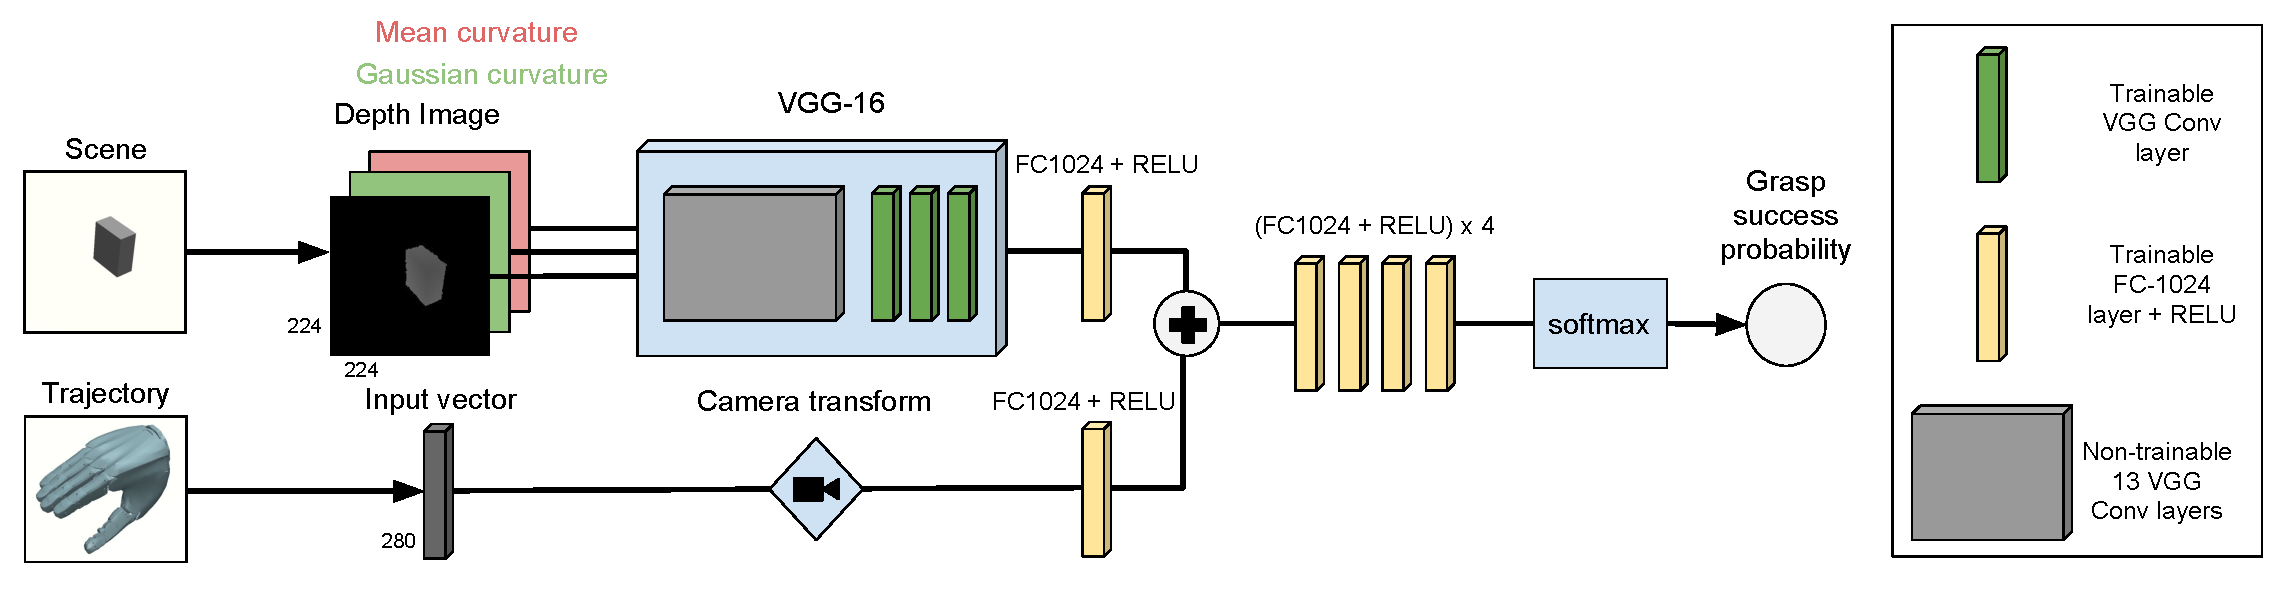
\includegraphics[width=0.95\textwidth]{images/networkArchitecture.pdf}
}
% \end{center}

% \begin{center}
\subfloat[new method 1]{%
    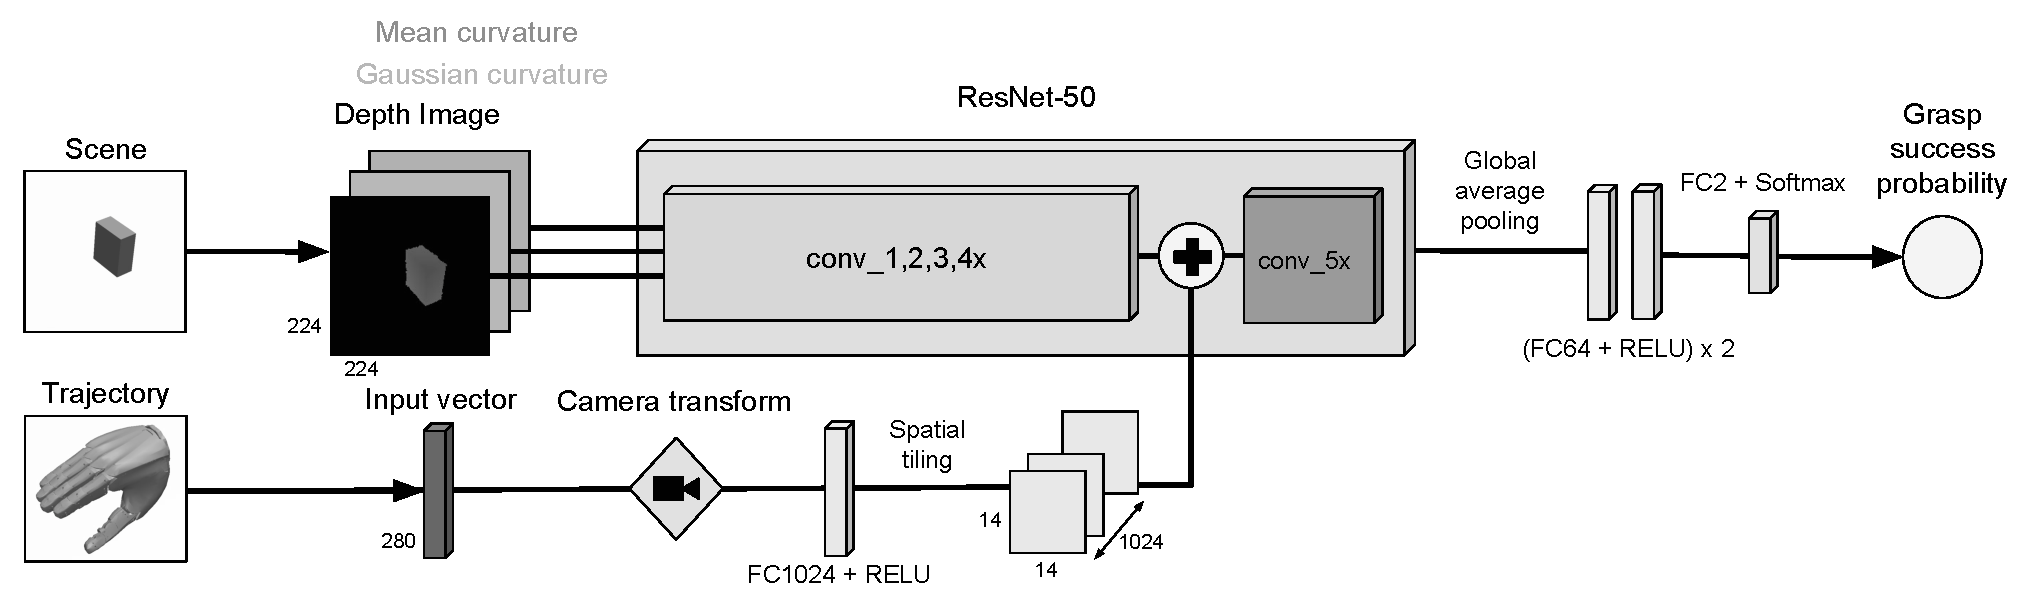
\includegraphics[width=0.85\textwidth]{images/ResNet.pdf}
}
% \end{center}

% \begin{center}
\subfloat[new method 2]{%
    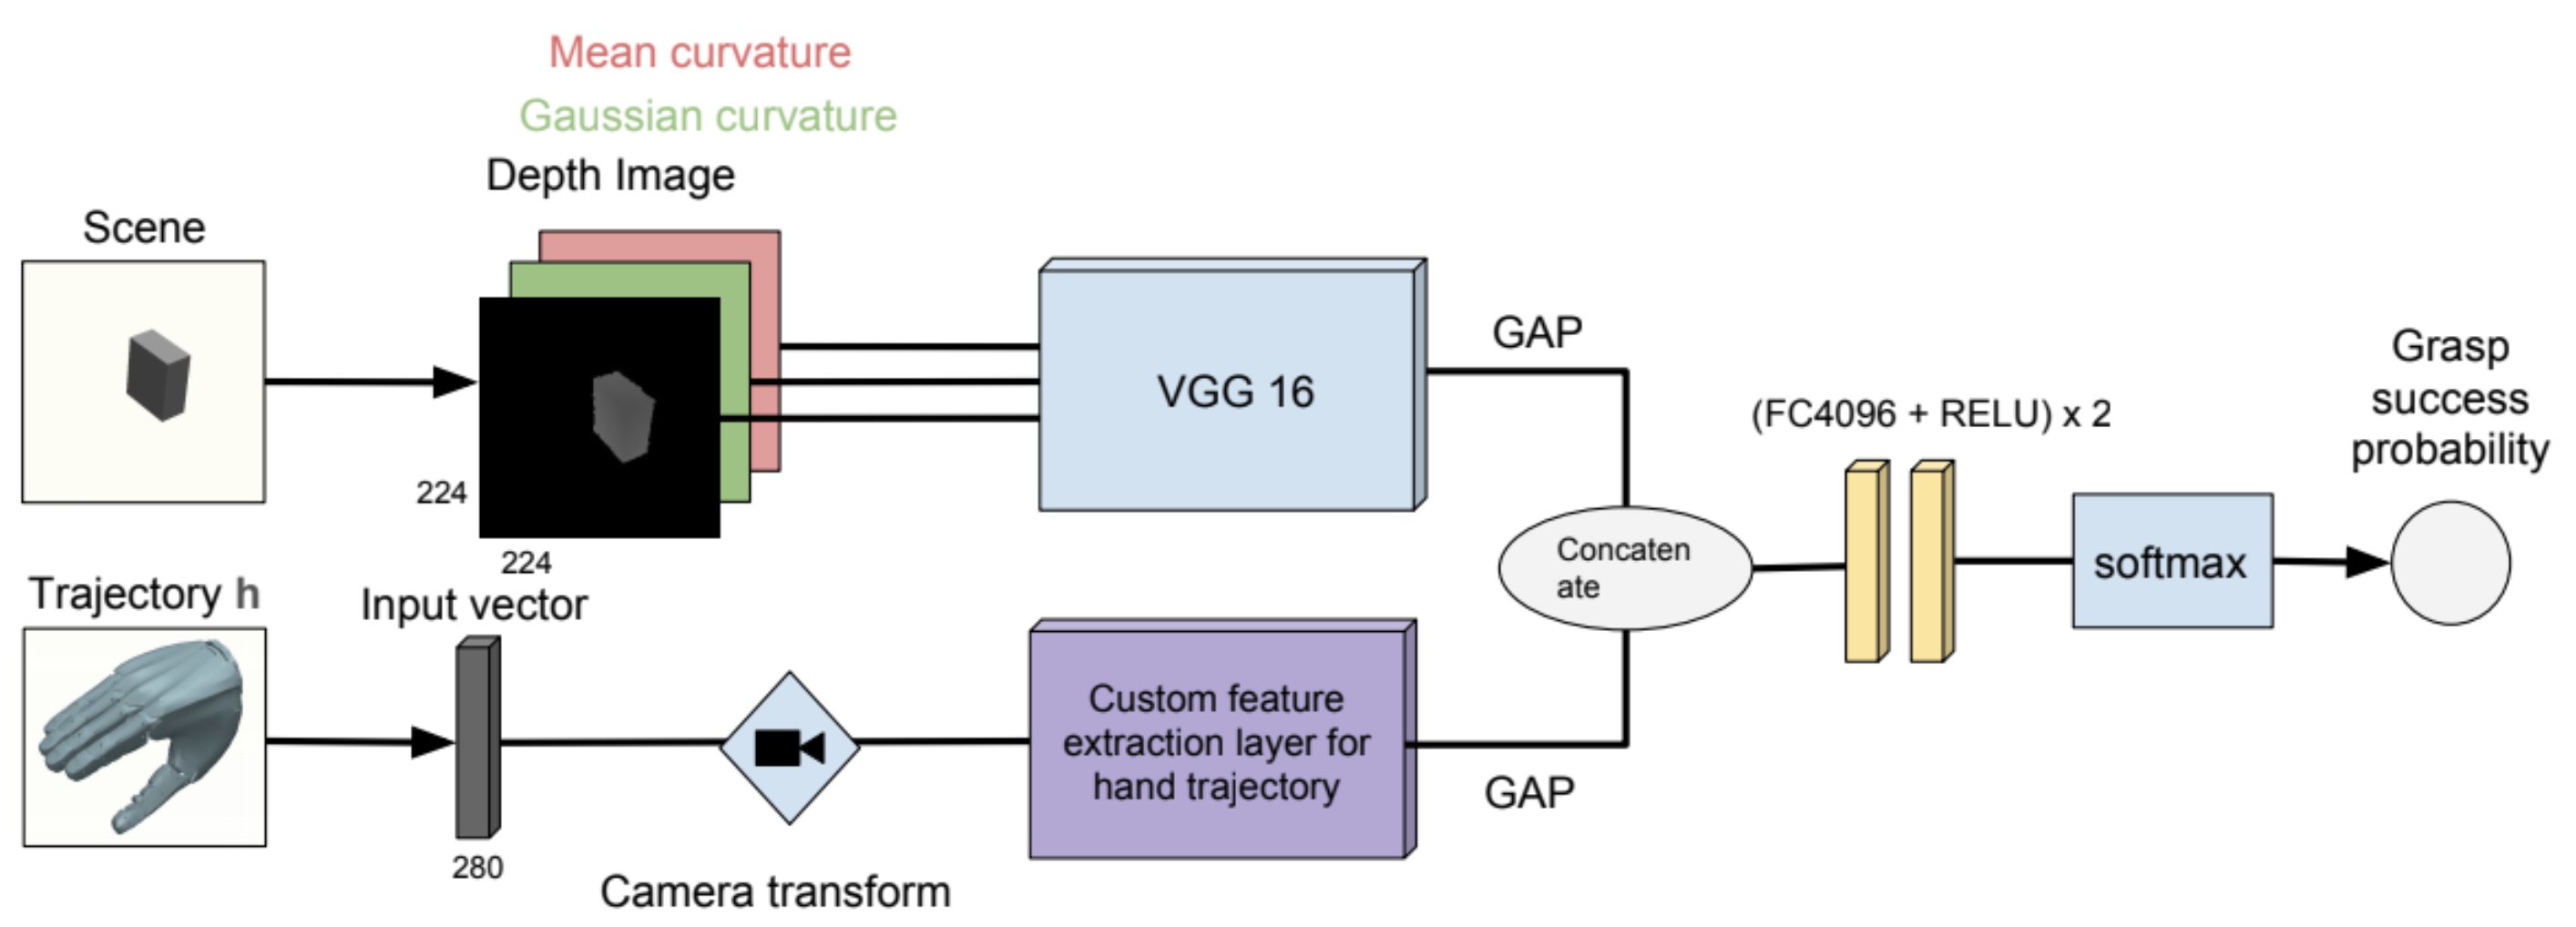
\includegraphics[width=0.75\textwidth]{images/ChaoNet.png}
}
% \end{center}

\caption{The three evaluative network architectures presented in this paper. Similarly to Levine et al. \cite{Levine1}, the two channels of information (visual data and grasp parameters) are processed in parallel and combined to reach the final decision in each model. RELU activations are used throughout the models, except for the final softmax layers. A final softmax layer has grasp success and and failure nodes, and learns to predict the success probability of a grasp. (a) VGG-16 based model in our previous paper \cite{icra}. The first 13 convolutional layers of VGG-16 are frozen. (b) ResNet50-based \cite{resnet} proposed network. The first four blocks are used for feature extraction, and the rest of the network is used to learn joint features. (c) VGG-16 based proposed model. The information pathways are joined via concatenation, not addition.}

\label{fig:networkArchitecture2}
\end{figure*}

% \begin{figure}[!ht]
% \subfloat{%
%   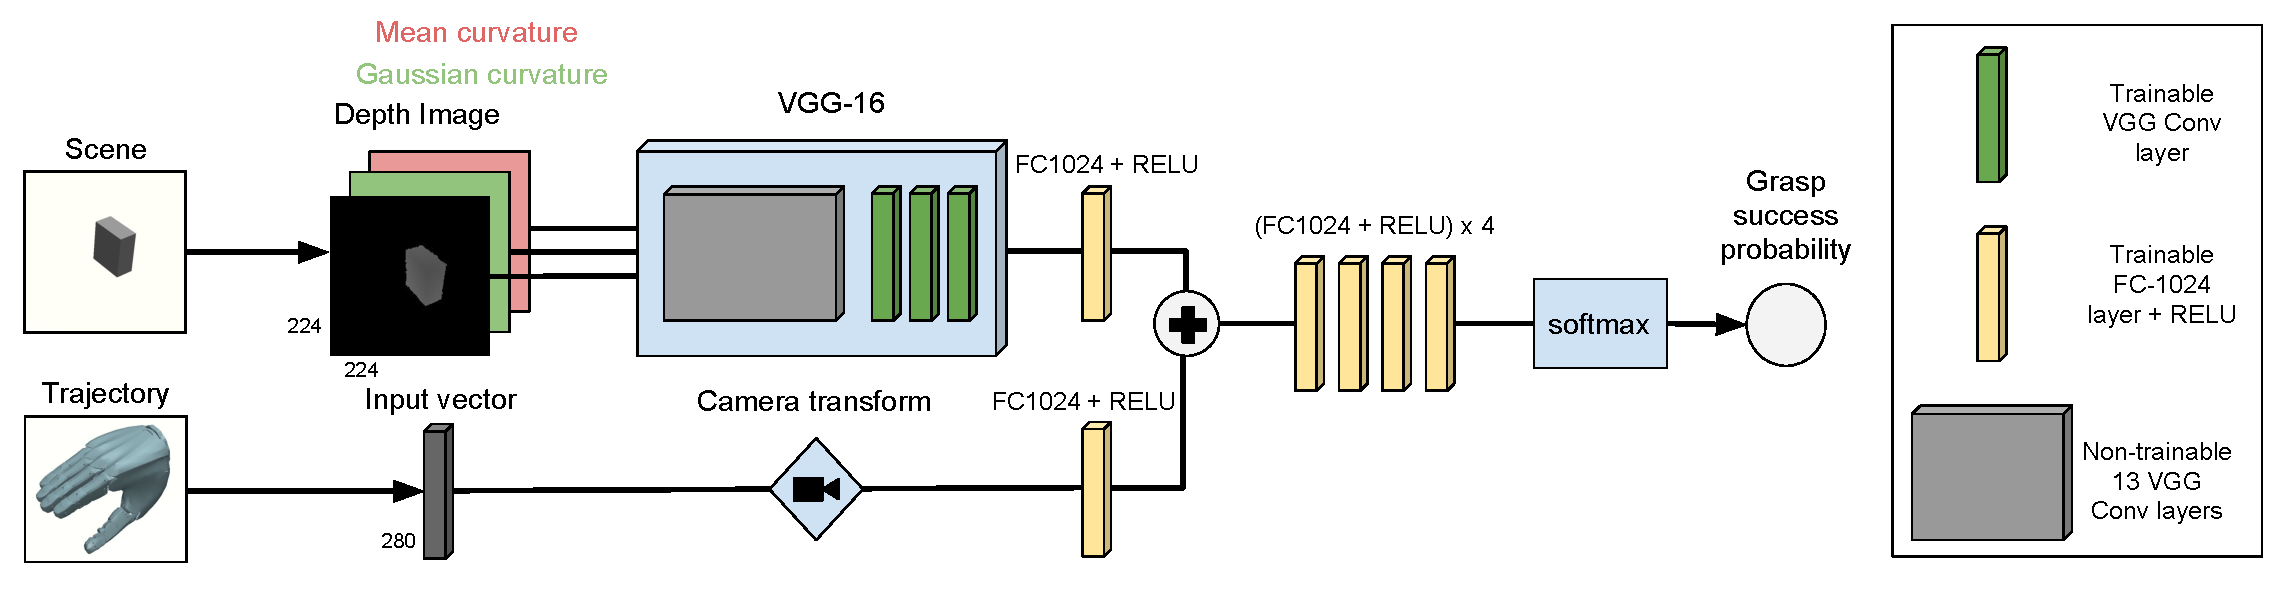
\includegraphics[width=0.9\textwidth]{images/networkArchitecture.pdf}
% }
% \caption[The VGG-16-based evaluative deep neural network architecture.]{The VGG-16-based evaluative deep neural network architecture. The first 13 convolutional layers of VGG-16 are not trained. Similarly to Levine et al. \cite{Levine1}, the two channels of information (grasp parameters and visual features) are joined via element-wise addition. The combined information is then passed through four fully-connected layers activated with RELU. The final softmax layer has grasp success and and failure nodes, and learns to predict the success probability of a grasp.}
% \subfloat{%
%     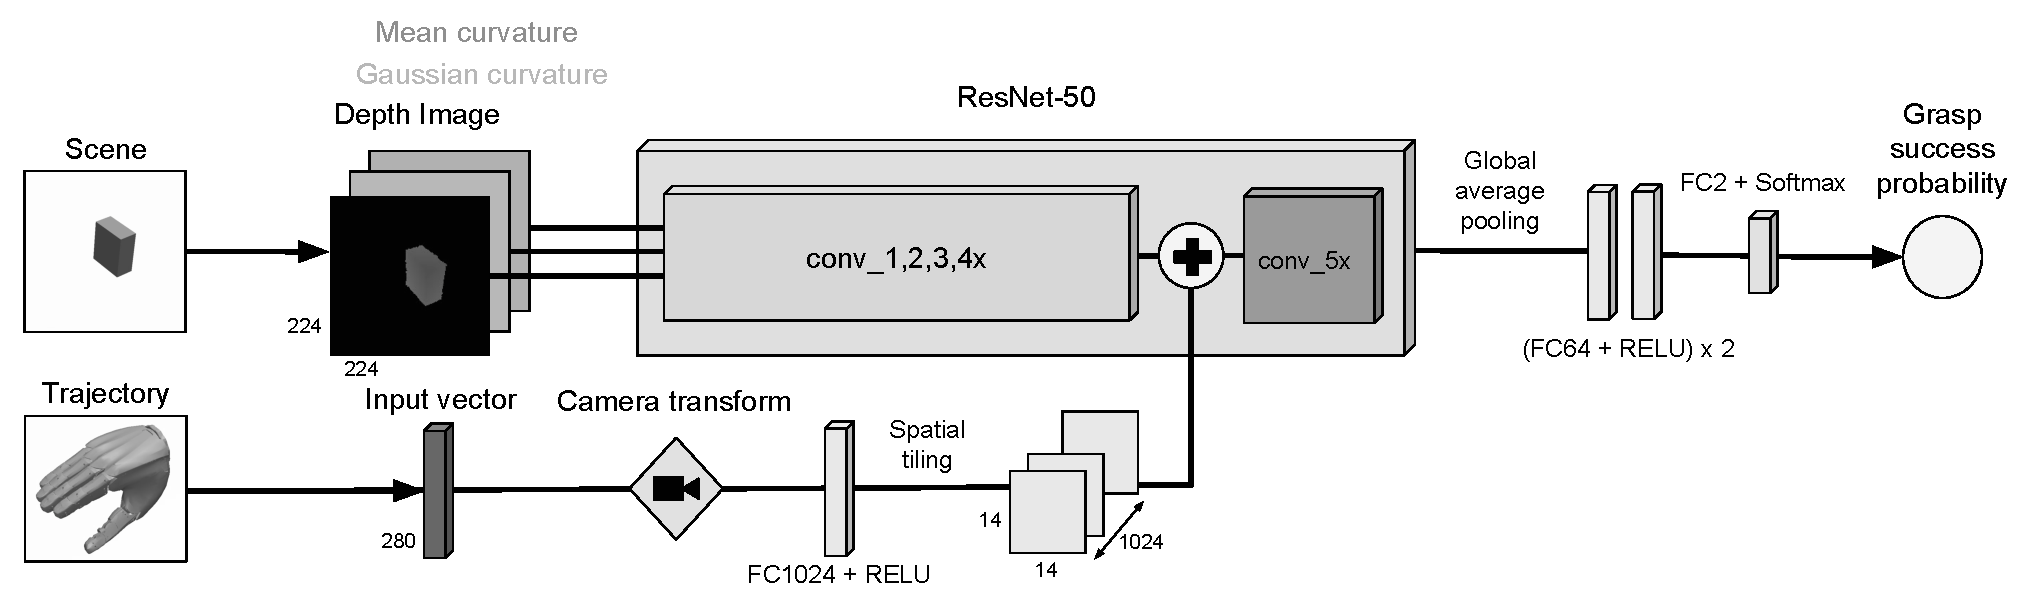
\includegraphics[width=0.9\textwidth]{images/ResNet.pdf}
%       \caption[The VGG-16-based evaluative deep neural network architecture.]{The VGG-16-based evaluative deep neural network architecture. The first 13 convolutional layers of VGG-16 are not trained. Similarly to Levine et al. \cite{Levine1}, the two channels of information (grasp parameters and visual features) are joined via element-wise addition. The combined information is then passed through four fully-connected layers activated with RELU. The final softmax layer has grasp success and and failure nodes, and learns to predict the success probability of a grasp.}
% }
% \subfloat{%
%   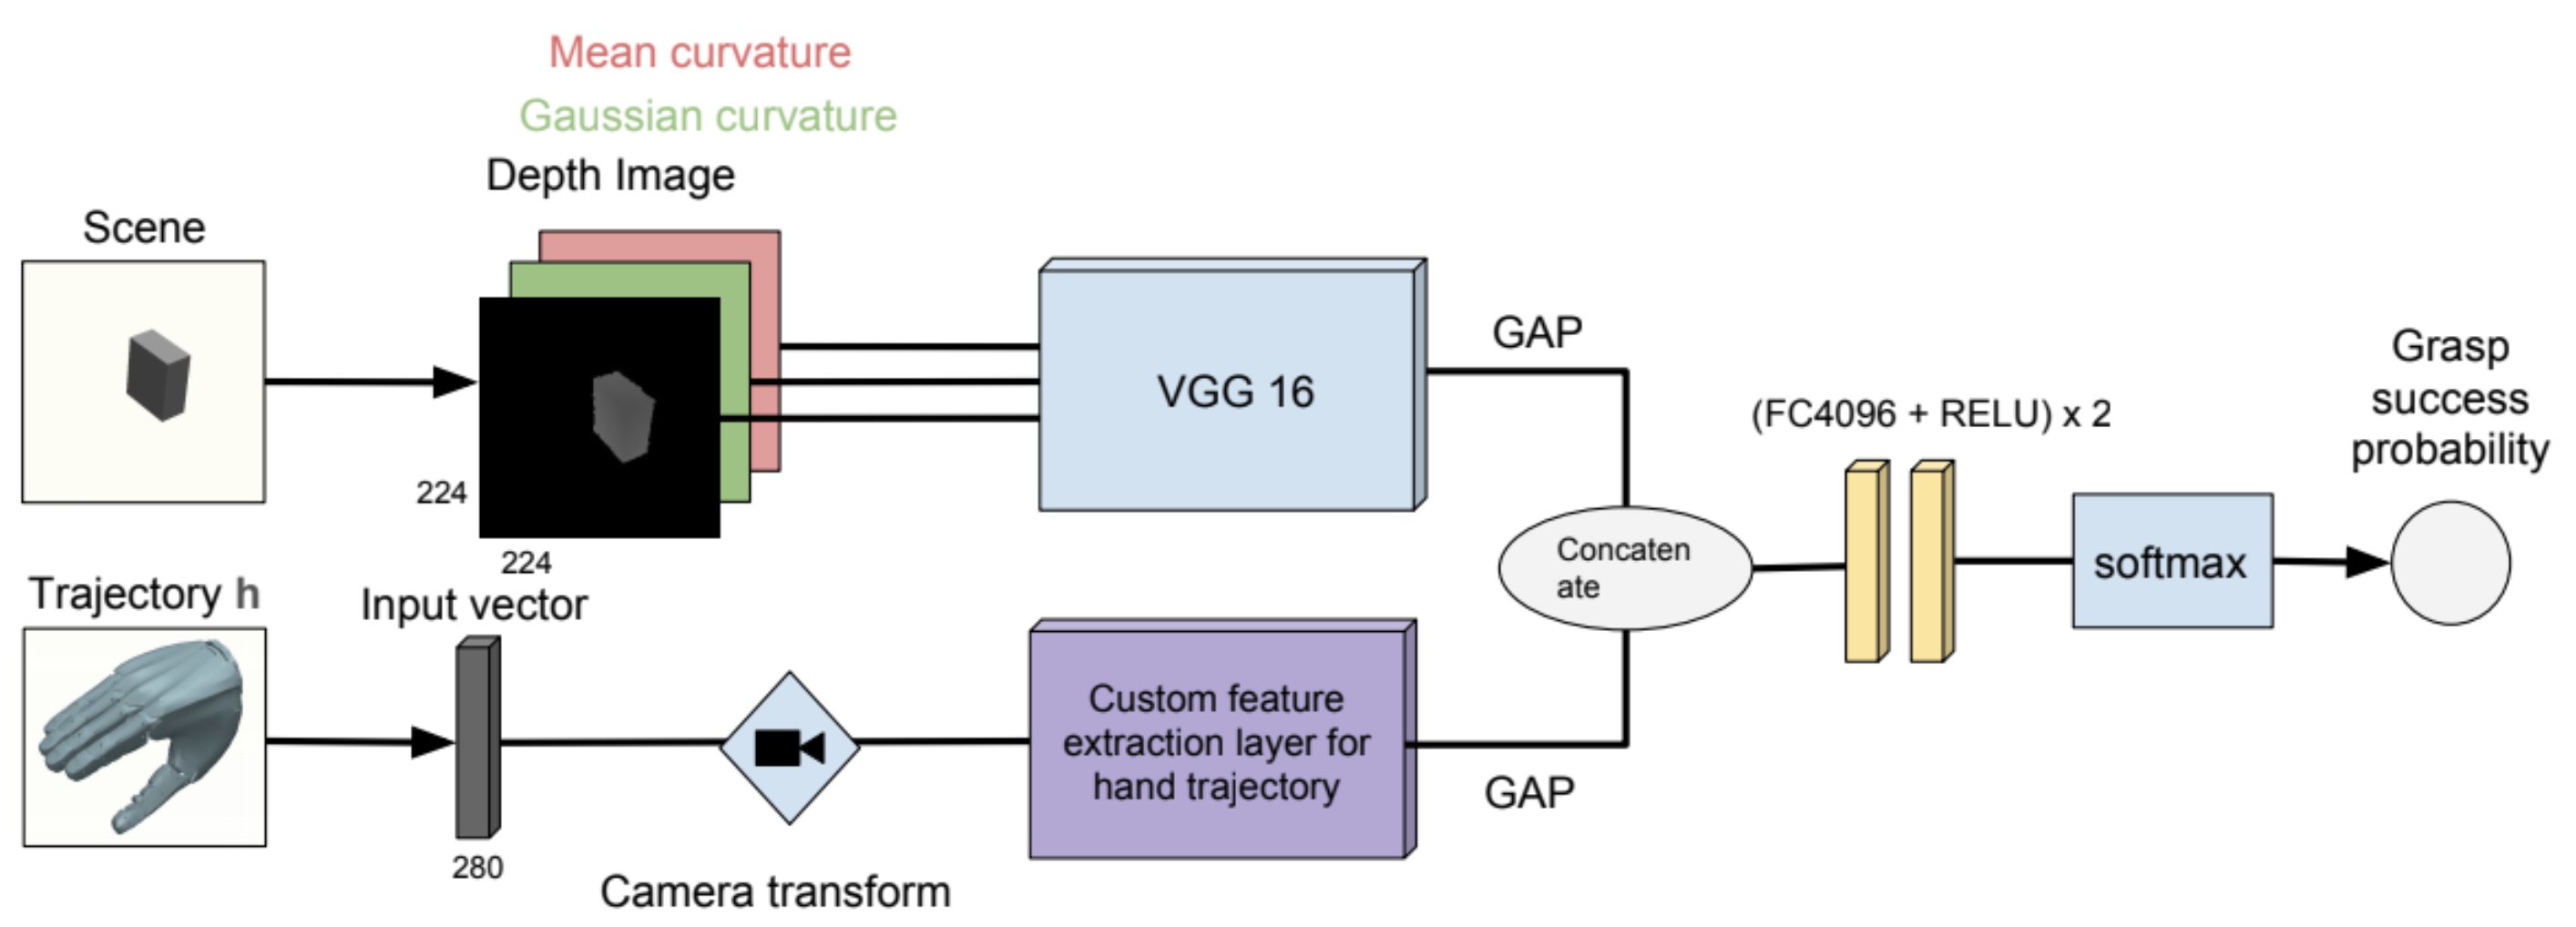
\includegraphics[width=0.9\textwidth]{images/ChaoNet.png}
%       \caption[The VGG-16-based evaluative deep neural network architecture.]{The VGG-16-based evaluative deep neural network architecture. The first 13 convolutional layers of VGG-16 are not trained. Similarly to Levine et al. \cite{Levine1}, the two channels of information (grasp parameters and visual features) are joined via element-wise addition. The combined information is then passed through four fully-connected layers activated with RELU. The final softmax layer has grasp success and and failure nodes, and learns to predict the success probability of a grasp.}
% }
% % \end{center}
% \label{fig:networkArchitecture}
% \end{figure}

Figure \ref{fig:networkArchitecture} demonstrates the architecture of the first proposed evaluative network. The colourised depth image is processed with the VGG-16 network \cite{Simonyan14c} to obtain the high-level image features. The VGG-16 network is initialised with the weights obtained from ImageNet training. Only the last three convolutional layers are trained, and the first 13 layers remain frozen. This decision was made in order to speed up training.

The grasp parameters and image features pass through fully-connected layers with 1024 hidden nodes (FC-1024) layers in order to obtain two feature vectors of length 1024. The features are combined using the element-wise addition operation, and are further processed using 4 FC-1024 layers. Similarly with \cite{Levine1}, the features are combined using addition and not concatenation. In this thesis, this decision was made based on the observation that addition yielded a marginally better performance in the experiments (not included in this thesis). Furthermore, concatenation and addition can be considered as interchangeable operations when combining different information pathways in deep networks \cite{dumoulin2018feature-wise}. The final FC-1024 layers form the associations between the visual features and hand parameters, and contain most of the parameters in the network. 

\subsection{Evaluative Model 2 (EM2)}

% \begin{figure}[!ht]
%   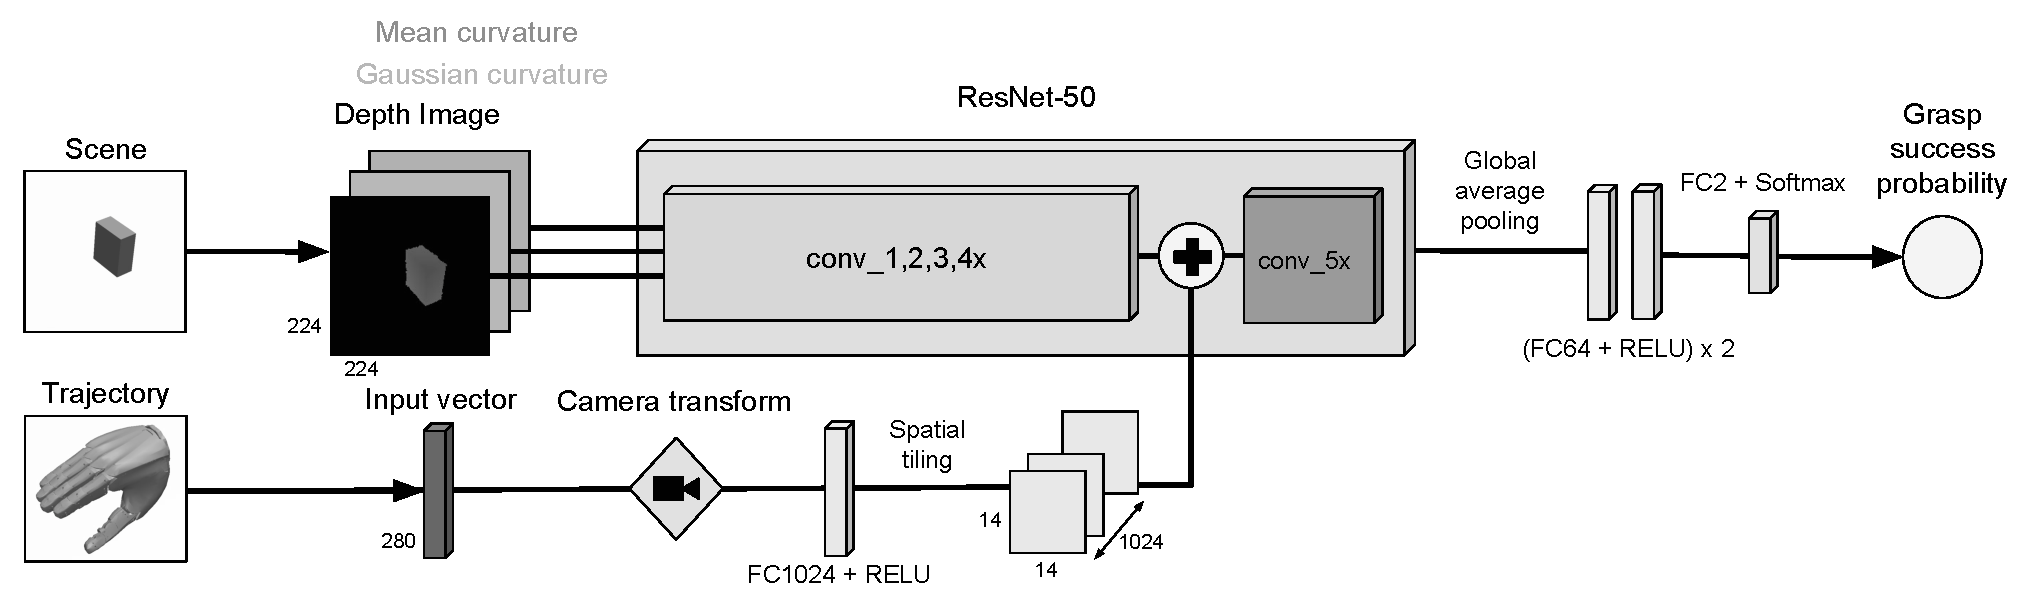
\includegraphics[width=\textwidth]{images/ResNet.pdf}
%   \caption[The ResNet-based evaluative deep neural network architecture.]{The ResNet-based evaluative deep neural network architecture (EM2). Spatial tiling is used to repeat the grasp parameters before they join the image processing pathway. This network requires fewer FC layers due to the earlier marriage of information channels.}
% \label{fig:ResNet}
% \end{figure}

The second evaluative model, termed EM2, uses the ResNet-50 network in order to obtain the high-level image features. Similarly with VGG-16, the ResNet-50 architecture is initialised with the weights that have been obtained during ImageNet training. One exception is the last convolution block conv\_5x, which is initialised randomly. In the EM2 architecture, ResNet-50 network is broken down into two parts: the first 4 convolutional blocks are used to extract the visual features. The final convolutional block, which has 9 convolutional layers, combines the image features and grasp parameters. Similarly with EM1, element-wise addition joins the two channels of information. Spatial tiling is used to convert the processed grasp parameters, a vector of size $1024$, to a matrix of size $14 \times 14 \times 1024$. Because the last convolutional block conv\_5x processes combined information, this network is designed with only 2 FC layers with 64 hidden nodes each. The output layer is the same as EM1. 

Both networks were trained on simulated data and tested on the real robot, as well as in simulation. The generative-evaluative architectures which use EM1 and EM2 are called GEA1 and GEA2, respectively. The next section focuses on the collection of the training data.